% Options for packages loaded elsewhere
\PassOptionsToPackage{unicode}{hyperref}
\PassOptionsToPackage{hyphens}{url}
%
\documentclass[
]{article}
\usepackage{amsmath,amssymb}
\usepackage{iftex}
\ifPDFTeX
  \usepackage[T1]{fontenc}
  \usepackage[utf8]{inputenc}
  \usepackage{textcomp} % provide euro and other symbols
\else % if luatex or xetex
  \usepackage{unicode-math} % this also loads fontspec
  \defaultfontfeatures{Scale=MatchLowercase}
  \defaultfontfeatures[\rmfamily]{Ligatures=TeX,Scale=1}
\fi
\usepackage{lmodern}
\ifPDFTeX\else
  % xetex/luatex font selection
\fi
% Use upquote if available, for straight quotes in verbatim environments
\IfFileExists{upquote.sty}{\usepackage{upquote}}{}
\IfFileExists{microtype.sty}{% use microtype if available
  \usepackage[]{microtype}
  \UseMicrotypeSet[protrusion]{basicmath} % disable protrusion for tt fonts
}{}
\makeatletter
\@ifundefined{KOMAClassName}{% if non-KOMA class
  \IfFileExists{parskip.sty}{%
    \usepackage{parskip}
  }{% else
    \setlength{\parindent}{0pt}
    \setlength{\parskip}{6pt plus 2pt minus 1pt}}
}{% if KOMA class
  \KOMAoptions{parskip=half}}
\makeatother
\usepackage{xcolor}
\usepackage[margin=1in]{geometry}
\usepackage{color}
\usepackage{fancyvrb}
\newcommand{\VerbBar}{|}
\newcommand{\VERB}{\Verb[commandchars=\\\{\}]}
\DefineVerbatimEnvironment{Highlighting}{Verbatim}{commandchars=\\\{\}}
% Add ',fontsize=\small' for more characters per line
\usepackage{framed}
\definecolor{shadecolor}{RGB}{248,248,248}
\newenvironment{Shaded}{\begin{snugshade}}{\end{snugshade}}
\newcommand{\AlertTok}[1]{\textcolor[rgb]{0.94,0.16,0.16}{#1}}
\newcommand{\AnnotationTok}[1]{\textcolor[rgb]{0.56,0.35,0.01}{\textbf{\textit{#1}}}}
\newcommand{\AttributeTok}[1]{\textcolor[rgb]{0.13,0.29,0.53}{#1}}
\newcommand{\BaseNTok}[1]{\textcolor[rgb]{0.00,0.00,0.81}{#1}}
\newcommand{\BuiltInTok}[1]{#1}
\newcommand{\CharTok}[1]{\textcolor[rgb]{0.31,0.60,0.02}{#1}}
\newcommand{\CommentTok}[1]{\textcolor[rgb]{0.56,0.35,0.01}{\textit{#1}}}
\newcommand{\CommentVarTok}[1]{\textcolor[rgb]{0.56,0.35,0.01}{\textbf{\textit{#1}}}}
\newcommand{\ConstantTok}[1]{\textcolor[rgb]{0.56,0.35,0.01}{#1}}
\newcommand{\ControlFlowTok}[1]{\textcolor[rgb]{0.13,0.29,0.53}{\textbf{#1}}}
\newcommand{\DataTypeTok}[1]{\textcolor[rgb]{0.13,0.29,0.53}{#1}}
\newcommand{\DecValTok}[1]{\textcolor[rgb]{0.00,0.00,0.81}{#1}}
\newcommand{\DocumentationTok}[1]{\textcolor[rgb]{0.56,0.35,0.01}{\textbf{\textit{#1}}}}
\newcommand{\ErrorTok}[1]{\textcolor[rgb]{0.64,0.00,0.00}{\textbf{#1}}}
\newcommand{\ExtensionTok}[1]{#1}
\newcommand{\FloatTok}[1]{\textcolor[rgb]{0.00,0.00,0.81}{#1}}
\newcommand{\FunctionTok}[1]{\textcolor[rgb]{0.13,0.29,0.53}{\textbf{#1}}}
\newcommand{\ImportTok}[1]{#1}
\newcommand{\InformationTok}[1]{\textcolor[rgb]{0.56,0.35,0.01}{\textbf{\textit{#1}}}}
\newcommand{\KeywordTok}[1]{\textcolor[rgb]{0.13,0.29,0.53}{\textbf{#1}}}
\newcommand{\NormalTok}[1]{#1}
\newcommand{\OperatorTok}[1]{\textcolor[rgb]{0.81,0.36,0.00}{\textbf{#1}}}
\newcommand{\OtherTok}[1]{\textcolor[rgb]{0.56,0.35,0.01}{#1}}
\newcommand{\PreprocessorTok}[1]{\textcolor[rgb]{0.56,0.35,0.01}{\textit{#1}}}
\newcommand{\RegionMarkerTok}[1]{#1}
\newcommand{\SpecialCharTok}[1]{\textcolor[rgb]{0.81,0.36,0.00}{\textbf{#1}}}
\newcommand{\SpecialStringTok}[1]{\textcolor[rgb]{0.31,0.60,0.02}{#1}}
\newcommand{\StringTok}[1]{\textcolor[rgb]{0.31,0.60,0.02}{#1}}
\newcommand{\VariableTok}[1]{\textcolor[rgb]{0.00,0.00,0.00}{#1}}
\newcommand{\VerbatimStringTok}[1]{\textcolor[rgb]{0.31,0.60,0.02}{#1}}
\newcommand{\WarningTok}[1]{\textcolor[rgb]{0.56,0.35,0.01}{\textbf{\textit{#1}}}}
\usepackage{longtable,booktabs,array}
\usepackage{calc} % for calculating minipage widths
% Correct order of tables after \paragraph or \subparagraph
\usepackage{etoolbox}
\makeatletter
\patchcmd\longtable{\par}{\if@noskipsec\mbox{}\fi\par}{}{}
\makeatother
% Allow footnotes in longtable head/foot
\IfFileExists{footnotehyper.sty}{\usepackage{footnotehyper}}{\usepackage{footnote}}
\makesavenoteenv{longtable}
\usepackage{graphicx}
\makeatletter
\def\maxwidth{\ifdim\Gin@nat@width>\linewidth\linewidth\else\Gin@nat@width\fi}
\def\maxheight{\ifdim\Gin@nat@height>\textheight\textheight\else\Gin@nat@height\fi}
\makeatother
% Scale images if necessary, so that they will not overflow the page
% margins by default, and it is still possible to overwrite the defaults
% using explicit options in \includegraphics[width, height, ...]{}
\setkeys{Gin}{width=\maxwidth,height=\maxheight,keepaspectratio}
% Set default figure placement to htbp
\makeatletter
\def\fps@figure{htbp}
\makeatother
\setlength{\emergencystretch}{3em} % prevent overfull lines
\providecommand{\tightlist}{%
  \setlength{\itemsep}{0pt}\setlength{\parskip}{0pt}}
\setcounter{secnumdepth}{-\maxdimen} % remove section numbering
\ifLuaTeX
  \usepackage{selnolig}  % disable illegal ligatures
\fi
\IfFileExists{bookmark.sty}{\usepackage{bookmark}}{\usepackage{hyperref}}
\IfFileExists{xurl.sty}{\usepackage{xurl}}{} % add URL line breaks if available
\urlstyle{same}
\hypersetup{
  pdftitle={STA108Project\_Gabe\&ELLIESUFFER},
  pdfauthor={Ellie Chareonsuphiphat},
  hidelinks,
  pdfcreator={LaTeX via pandoc}}

\title{STA108Project\_Gabe\&ELLIESUFFER}
\author{Ellie Chareonsuphiphat}
\date{2023-11-23}

\begin{document}
\maketitle

\begin{verbatim}
## 
## Attaching package: 'dplyr'
\end{verbatim}

\begin{verbatim}
## The following objects are masked from 'package:stats':
## 
##     filter, lag
\end{verbatim}

\begin{verbatim}
## The following objects are masked from 'package:base':
## 
##     intersect, setdiff, setequal, union
\end{verbatim}

\begin{verbatim}
## 
## Attaching package: 'MASS'
\end{verbatim}

\begin{verbatim}
## The following object is masked from 'package:dplyr':
## 
##     select
\end{verbatim}

\begin{verbatim}
## Warning: package 'leaps' was built under R version 4.3.2
\end{verbatim}

\begin{Shaded}
\begin{Highlighting}[]
\CommentTok{\# Load Data}
\NormalTok{countries }\OtherTok{\textless{}{-}} \FunctionTok{read.csv}\NormalTok{(}\StringTok{"../countries.csv"}\NormalTok{)}
\NormalTok{countries }\OtherTok{\textless{}{-}}\NormalTok{ janitor}\SpecialCharTok{::}\FunctionTok{clean\_names}\NormalTok{(countries)}
\end{Highlighting}
\end{Shaded}

\hypertarget{single-linear-regression-models}{%
\subsection{Single Linear Regression
Models}\label{single-linear-regression-models}}

Create a single linear regression model for life expectancy
\textasciitilde{} X. Generate all necessary plots for regression
analysis.

Variables to change: Note: All variables that need to be changed will
have a ``\#'' next to the line of code - x.lab : Name of X variable.
Capitalize the first letter, use full names, use space instead of
``\_``. (Ex. land\_area -\textgreater{} Land Area) - x.dat : Linear
Model X variable - Linear Model Names: Name of X variable followed
by''\_lm'' and ``\_lm\_summary'' respectively. - The corresponding
variable name in the ``\#Display Values'' section

\textbf{Life Expectancy \textasciitilde{} Land Area}

\begin{Shaded}
\begin{Highlighting}[]
\CommentTok{\# Variable Names}
\NormalTok{x.lab }\OtherTok{\textless{}{-}} \StringTok{"Land Area"} \CommentTok{\#\textless{}change\textgreater{}}
\NormalTok{x.dat }\OtherTok{\textless{}{-}}\NormalTok{ countries}\SpecialCharTok{$}\NormalTok{land\_area }\CommentTok{\#\textless{}change\textgreater{}}

\NormalTok{y.lab }\OtherTok{\textless{}{-}} \StringTok{"Life Expectancy"}
\NormalTok{title }\OtherTok{\textless{}{-}} \FunctionTok{paste}\NormalTok{(y.lab, }\StringTok{"\textasciitilde{}"}\NormalTok{, x.lab)}
  
\CommentTok{\# Create Linear Model}
\NormalTok{landarea\_lm }\OtherTok{\textless{}{-}} \FunctionTok{lm}\NormalTok{(life\_expectancy }\SpecialCharTok{\textasciitilde{}}\NormalTok{ x.dat, }\AttributeTok{data=}\NormalTok{countries, ) }\CommentTok{\#\textless{}change\textgreater{}}
\NormalTok{landarea\_lm\_summary }\OtherTok{\textless{}{-}} \FunctionTok{summary}\NormalTok{(landarea\_lm) }\CommentTok{\#\textless{}change\textgreater{}}
\FunctionTok{row.names}\NormalTok{(landarea\_lm\_summary}\SpecialCharTok{$}\NormalTok{coefficients) }\OtherTok{\textless{}{-}} \FunctionTok{c}\NormalTok{(}\StringTok{"(Intercept)"}\NormalTok{, x.lab) }\CommentTok{\#\textless{}change\textgreater{}}

\CommentTok{\# Display Values}
\FunctionTok{kable}\NormalTok{(landarea\_lm\_summary}\SpecialCharTok{$}\NormalTok{coefficients, }\CommentTok{\#\textless{}change\textgreater{}}
      \AttributeTok{caption=}\NormalTok{title)}
\end{Highlighting}
\end{Shaded}

\begin{longtable}[]{@{}lrrrr@{}}
\caption{Life Expectancy \textasciitilde{} Land Area}\tabularnewline
\toprule\noalign{}
& Estimate & Std. Error & t value &
Pr(\textgreater\textbar t\textbar) \\
\midrule\noalign{}
\endfirsthead
\toprule\noalign{}
& Estimate & Std. Error & t value &
Pr(\textgreater\textbar t\textbar) \\
\midrule\noalign{}
\endhead
\bottomrule\noalign{}
\endlastfoot
(Intercept) & 68.4102866 & 0.8068269 & 84.789303 & 0.0000000 \\
Land Area & 0.0000002 & 0.0000004 & 0.379057 & 0.7050826 \\
\end{longtable}

\begin{Shaded}
\begin{Highlighting}[]
\CommentTok{\# Scatterplot}
\NormalTok{landarea\_scatter }\OtherTok{\textless{}{-}}\NormalTok{ countries}\SpecialCharTok{\%\textgreater{}\%} \CommentTok{\#\textless{}change\textgreater{}}
  \FunctionTok{ggplot}\NormalTok{(}\FunctionTok{aes}\NormalTok{(}\AttributeTok{y=}\NormalTok{life\_expectancy, }
             \AttributeTok{x=}\NormalTok{x.dat))}\SpecialCharTok{+}
  \FunctionTok{geom\_point}\NormalTok{(}\AttributeTok{color=}\StringTok{\textquotesingle{}cyan4\textquotesingle{}}\NormalTok{)}\SpecialCharTok{+}
  \FunctionTok{geom\_smooth}\NormalTok{(}\AttributeTok{method=}\StringTok{\textquotesingle{}lm\textquotesingle{}}\NormalTok{, }\AttributeTok{color=}\StringTok{"black"}\NormalTok{)}\SpecialCharTok{+}
  \FunctionTok{labs}\NormalTok{(}\AttributeTok{title=}\NormalTok{title,}
       \AttributeTok{x=}\NormalTok{x.lab,}
       \AttributeTok{y=}\NormalTok{y.lab)}\SpecialCharTok{+}
  \FunctionTok{theme\_light}\NormalTok{()}
\FunctionTok{ggsave}\NormalTok{(}\AttributeTok{filename=}\FunctionTok{paste}\NormalTok{(x.lab, }\StringTok{"Scatterplot.png"}\NormalTok{), }\AttributeTok{device =} \StringTok{"png"}\NormalTok{, }\AttributeTok{path=}\FunctionTok{paste0}\NormalTok{(}\StringTok{"../Plots/"}\NormalTok{, x.lab))}
\end{Highlighting}
\end{Shaded}

\begin{verbatim}
## Saving 6.5 x 4.5 in image
## `geom_smooth()` using formula = 'y ~ x'
\end{verbatim}

\begin{Shaded}
\begin{Highlighting}[]
\CommentTok{\# Residual Plot}
\NormalTok{landarea\_resid }\OtherTok{\textless{}{-}}\NormalTok{ countries}\SpecialCharTok{\%\textgreater{}\%}  \CommentTok{\#\textless{}change\textgreater{}}
  \FunctionTok{ggplot}\NormalTok{(}\FunctionTok{aes}\NormalTok{(}\AttributeTok{x=}\FunctionTok{fitted}\NormalTok{(landarea\_lm), }\CommentTok{\#\textless{}change\textgreater{}}
             \AttributeTok{y=}\FunctionTok{residuals}\NormalTok{(landarea\_lm) }\CommentTok{\#\textless{}change\textgreater{}}
\NormalTok{             ))}\SpecialCharTok{+}
  \FunctionTok{geom\_point}\NormalTok{(}\AttributeTok{color=}\StringTok{"darkgoldenrod"}\NormalTok{, }\AttributeTok{shape=}\DecValTok{21}\NormalTok{)}\SpecialCharTok{+}
  \FunctionTok{geom\_hline}\NormalTok{(}\AttributeTok{yintercept=}\DecValTok{0}\NormalTok{)}\SpecialCharTok{+}
  \FunctionTok{labs}\NormalTok{(}\AttributeTok{title=}\StringTok{"Residuals Against Fitted Values"}\NormalTok{,}
       \AttributeTok{x=}\StringTok{"Fitted Values"}\NormalTok{,}
       \AttributeTok{y=}\StringTok{"Residuals"}\NormalTok{)}
\FunctionTok{ggsave}\NormalTok{(}\AttributeTok{filename=}\FunctionTok{paste}\NormalTok{(x.lab, }\StringTok{"Residual Plot.png"}\NormalTok{), }\AttributeTok{device =} \StringTok{"png"}\NormalTok{, }\AttributeTok{path=}\FunctionTok{paste0}\NormalTok{(}\StringTok{"../Plots/"}\NormalTok{, x.lab))}
\end{Highlighting}
\end{Shaded}

\begin{verbatim}
## Saving 6.5 x 4.5 in image
\end{verbatim}

\begin{Shaded}
\begin{Highlighting}[]
\CommentTok{\# Residual QQ Plot}
\NormalTok{landarea\_ResidQQ }\OtherTok{\textless{}{-}}\NormalTok{ landarea\_lm}\SpecialCharTok{\%\textgreater{}\%} \CommentTok{\#\textless{}change\textgreater{}}
  \FunctionTok{ggplot}\NormalTok{(}\FunctionTok{aes}\NormalTok{(}\AttributeTok{sample=}\FunctionTok{residuals}\NormalTok{(landarea\_lm)))}\SpecialCharTok{+} \CommentTok{\#\textless{}change\textgreater{}}
  \FunctionTok{geom\_qq}\NormalTok{(}\AttributeTok{color=}\StringTok{"brown3"}\NormalTok{, }\AttributeTok{size=}\FloatTok{1.3}\NormalTok{)}\SpecialCharTok{+}
  \FunctionTok{geom\_qq\_line}\NormalTok{()}\SpecialCharTok{+}
  \FunctionTok{labs}\NormalTok{(}\AttributeTok{title=}\StringTok{"Residual QQ Plot"}\NormalTok{,}
       \AttributeTok{x=}\StringTok{"Theoretical Quantiles"}\NormalTok{,}
       \AttributeTok{y=}\StringTok{"Sample Quantiles"}\NormalTok{)}
\FunctionTok{ggsave}\NormalTok{(}\AttributeTok{filename=}\FunctionTok{paste}\NormalTok{(}\StringTok{"Residual QQ Plot.png"}\NormalTok{), }\AttributeTok{device =} \StringTok{"png"}\NormalTok{, }\AttributeTok{path=}\FunctionTok{paste0}\NormalTok{(}\StringTok{"../Plots/"}\NormalTok{, x.lab))}
\end{Highlighting}
\end{Shaded}

\begin{verbatim}
## Saving 6.5 x 4.5 in image
\end{verbatim}

\begin{Shaded}
\begin{Highlighting}[]
\CommentTok{\# Predictor QQ Plot}
\NormalTok{landarea\_QQ }\OtherTok{\textless{}{-}}\NormalTok{ landarea\_lm}\SpecialCharTok{\%\textgreater{}\%} \CommentTok{\#\textless{}change\textgreater{}}
  \FunctionTok{ggplot}\NormalTok{(}\FunctionTok{aes}\NormalTok{(}\AttributeTok{sample=}\NormalTok{x.dat))}\SpecialCharTok{+}
  \FunctionTok{geom\_qq}\NormalTok{(}\AttributeTok{color=}\StringTok{"forestgreen"}\NormalTok{, }\AttributeTok{size=}\FloatTok{1.3}\NormalTok{)}\SpecialCharTok{+}
  \FunctionTok{geom\_qq\_line}\NormalTok{()}\SpecialCharTok{+}
  \FunctionTok{labs}\NormalTok{(}\AttributeTok{title=}\FunctionTok{paste}\NormalTok{(x.lab, }\StringTok{"QQ Plot"}\NormalTok{),}
       \AttributeTok{x=}\StringTok{"Theoretical Quantiles"}\NormalTok{,}
       \AttributeTok{y=}\StringTok{"Sample Quantiles"}\NormalTok{)}
\FunctionTok{ggsave}\NormalTok{(}\AttributeTok{filename=}\FunctionTok{paste}\NormalTok{(x.lab, }\StringTok{"QQ Plot.png"}\NormalTok{), }\AttributeTok{device =} \StringTok{"png"}\NormalTok{, }\AttributeTok{path=}\FunctionTok{paste0}\NormalTok{(}\StringTok{"../Plots/"}\NormalTok{, x.lab))}
\end{Highlighting}
\end{Shaded}

\begin{verbatim}
## Saving 6.5 x 4.5 in image
\end{verbatim}

\begin{Shaded}
\begin{Highlighting}[]
\FunctionTok{ggarrange}\NormalTok{(landarea\_scatter, landarea\_resid) }\CommentTok{\#\textless{}change\textgreater{}}
\end{Highlighting}
\end{Shaded}

\begin{verbatim}
## `geom_smooth()` using formula = 'y ~ x'
\end{verbatim}

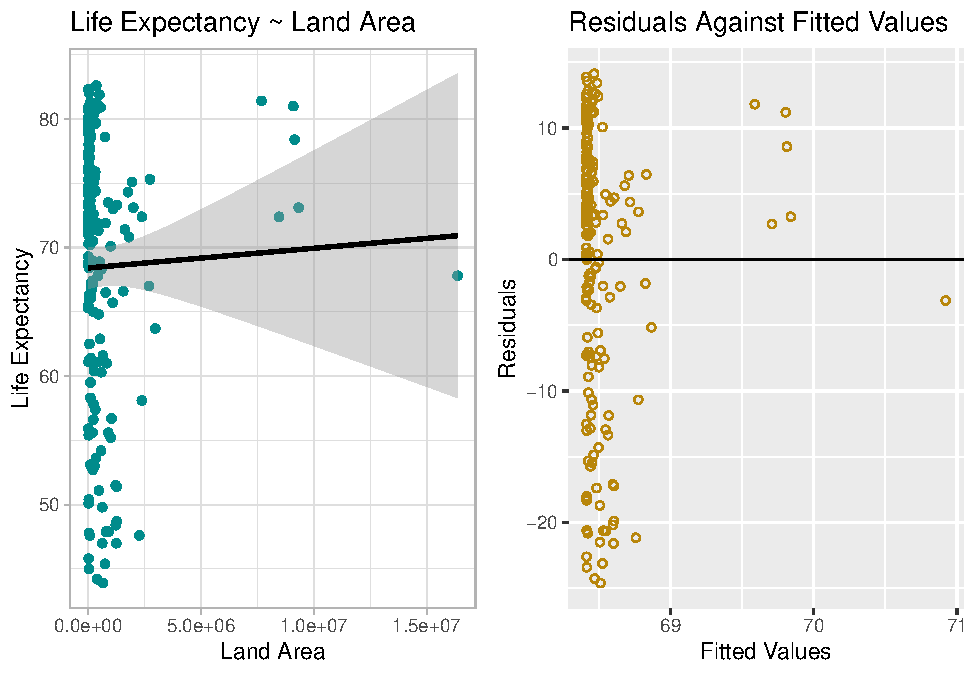
\includegraphics{STA108_TermProject_Jones-Chareonsuphiphat_files/figure-latex/unnamed-chunk-3-1.pdf}

\begin{Shaded}
\begin{Highlighting}[]
\FunctionTok{ggarrange}\NormalTok{(landarea\_QQ, landarea\_ResidQQ) }\CommentTok{\#\textless{}change\textgreater{}}
\end{Highlighting}
\end{Shaded}

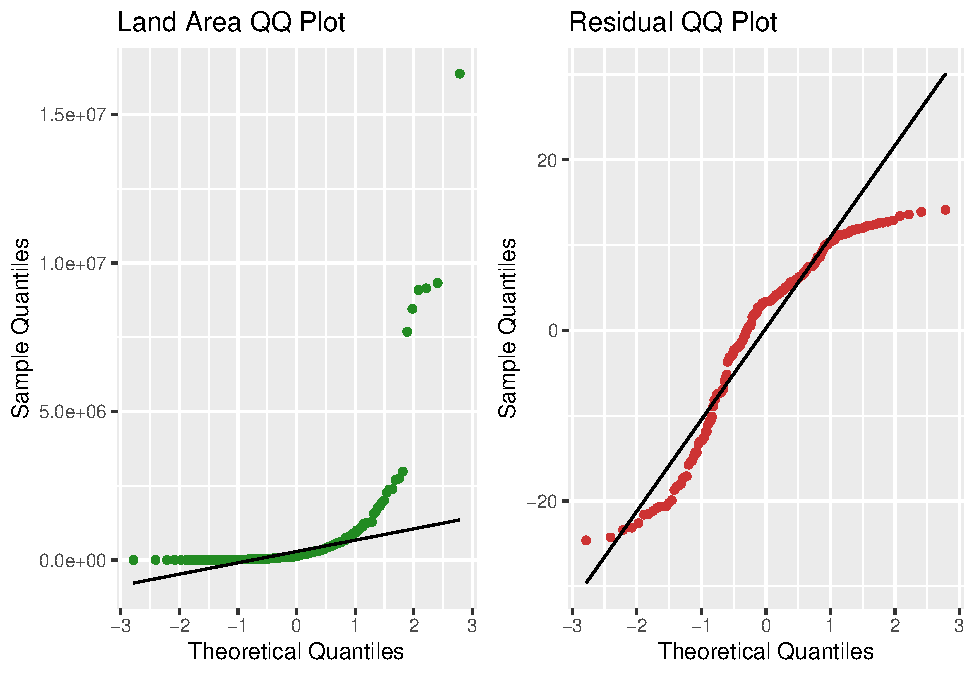
\includegraphics{STA108_TermProject_Jones-Chareonsuphiphat_files/figure-latex/unnamed-chunk-3-2.pdf}

\end{document}
